\documentclass[12pt]{article}
\usepackage{../preamble3}
%\pagenumbering{gobble}
\title{MathCounts Competition Practice IV, January 2021 \\ Sprint Round}
\author{Patrick \& James Toche}
\date{Revised:~\today}

\begin{document}
\maketitle
\begin{minipage}{\textwidth}
\begin{abstract}\setlength{\parindent}{0pt}%
Notes on Sprint Round of MathCounts Competition Practice IV, January 2021. 
Questions are from MathCounts Foundation (\url{https://www.mathcounts.org/}). Copyright restrictions may apply. Written for personal use. 
Please report typos and errors over at \url{https://github.com/ptoche/Math/tree/master/mathcounts}. 
\end{abstract}
\end{minipage}

\thispagestyle{empty}
\clearpage
\addtocounter{page}{-1}

\section*{Sprint Round}


%%%%%%%%%%%%%%%%%%%%%%%%%%%%%%%%%%%%%%%%%%%%%%%%%%%%%%%%%%%%%%%%%%%%%%%%
\subsection*{1.}
Raquel has collected $\$3.80$ in nickels and dimes. She has exactly $48$ nickels. How many dimes does she have?

\nopagebreak

\fbox{\phantom{ANSWER}}~dimes

\begin{answer}
\begin{tikzpicture}\node[textbox]{%
    \begin{minipagex}{\dimexpr\textwidth-20pt}
        A nickel is worth $\$0.05$. A dime is worth $\$0.10$.
        \begin{align*}
        3.80 - 48 \times 0.05 
        & = 3.80 - 2.40 \\
        & = 1.40 \\
        & = 14 \times 0.10
        \end{align*}
        \begin{empheq}[box={\mathbox[colback=white]}]{equation*}
            14 ~\text{dimes}
        \end{empheq}
    \end{minipagex}
    };
\end{tikzpicture}%
\end{answer}
%%%%%%%%%%%%%%%%%%%%%%%%%%%%%%%%%%%%%%%%%%%%%%%%%%%%%%%%%%%%%%%%%%%%%%%%


%%%%%%%%%%%%%%%%%%%%%%%%%%%%%%%%%%%%%%%%%%%%%%%%%%%%%%%%%%%%%%%%%%%%%%%%
\subsection*{2.}
At a certain middle school, there are $16$ seventh graders and $24$ eighth graders enrolled in algebra this term. What percent of the students enrolled in algebra are eighth graders?

\nopagebreak

\fbox{\phantom{ANSWER}}~\%

\begin{answer}
\begin{tikzpicture}\node[textbox]{%
    \begin{minipagex}{\dimexpr\textwidth-20pt}
        There are $40$ students, $24$ of which are eighth graders:
        \begin{align*}
        \frac{24}{16+24} = \frac{24}{40} = \frac{6}{10} = \frac{60}{100}
        \end{align*}
        \begin{empheq}[box={\mathbox[colback=white]}]{equation*}
            60\%
        \end{empheq}
    \end{minipagex}
    };
\end{tikzpicture}%
\end{answer}
%%%%%%%%%%%%%%%%%%%%%%%%%%%%%%%%%%%%%%%%%%%%%%%%%%%%%%%%%%%%%%%%%%%%%%%%



%%%%%%%%%%%%%%%%%%%%%%%%%%%%%%%%%%%%%%%%%%%%%%%%%%%%%%%%%%%%%%%%%%%%%%%%
\subsection*{3.}
What positive integer is $56$ less than its square?

\nopagebreak

\fbox{\phantom{ANSWER}}

\begin{answer}
\begin{tikzpicture}\node[textbox]{%
    \begin{minipagex}{\dimexpr\textwidth-20pt}
        Find $x\in\mathbb{N}$ such that
        \begin{align*}
        x^2 - 56 = x
        \end{align*}
        We know the solution is a positive integer, so we can make a quick guess: $x=10$ is obviously too large, but $x=8$ works. 
        Alternatively, solving the quadratic equation yields:
        \begin{align*}
        x_{1,2} = \frac{+1\pm \sqrt{1 + 4 \cdot 56}}{2} = \frac{+1\pm \sqrt{225}}{2} = \frac{+1\pm15}{2} = -7,8
        \end{align*}
        The positive integer is:
        \begin{empheq}[box={\mathbox[colback=white]}]{equation*}
            8
        \end{empheq}
    \end{minipagex}
    };
\end{tikzpicture}%
\end{answer}
%%%%%%%%%%%%%%%%%%%%%%%%%%%%%%%%%%%%%%%%%%%%%%%%%%%%%%%%%%%%%%%%%%%%%%%%



%%%%%%%%%%%%%%%%%%%%%%%%%%%%%%%%%%%%%%%%%%%%%%%%%%%%%%%%%%%%%%%%%%%%%%%%
\subsection*{4.}
Each year a certain tree doubled in height. At the end of $6$ years, the height of the tree was 32 feet. What was the height of the tree at the end of $3$ years?

\nopagebreak

\fbox{\phantom{ANSWER}}~feet

\begin{answer}
\begin{tikzpicture}\node[textbox]{%
    \begin{minipagex}{\dimexpr\textwidth-20pt}
        The problem defines the following recurrence:
        \begin{align*}
        h_{t} & = 2 h_{t-1} \\
        h_{6} & = 32
        \end{align*}
        We want to calculate $h_{3}$ knowing $h_{6}$. To go backwards $3$ steps, we need to divide $h_{6}$ by $2^{3}$:
        \begin{align*}
        h_{3} & = \frac{h_{6}}{2^{3}}
              = \frac{32}{8}
              = 4
        \end{align*}
        The height was:
        \begin{empheq}[box={\mathbox[colback=white]}]{equation*}
            4 ~\text{feet}
        \end{empheq}
    \end{minipagex}
    };
\end{tikzpicture}%
\end{answer}
%%%%%%%%%%%%%%%%%%%%%%%%%%%%%%%%%%%%%%%%%%%%%%%%%%%%%%%%%%%%%%%%%%%%%%%%



%%%%%%%%%%%%%%%%%%%%%%%%%%%%%%%%%%%%%%%%%%%%%%%%%%%%%%%%%%%%%%%%%%%%%%%%
\subsection*{5.}
If a certain recipe requires $5$ tablespoons of flour for every $2$ ounces of butter, how many tablespoons of flour are needed if $2$ pounds of butter are used? There are $16$ ounces of butter in one pound. 

\nopagebreak

\fbox{\phantom{ANSWER}}~tablespoons

\begin{answer}
\begin{tikzpicture}\node[textbox]{%
    \begin{minipagex}{\dimexpr\textwidth-20pt}
        Since $1$ pound is equivalent to $16$ ounces, then the $2$ pounds needed are equivalent to $32$ ounces. We need to convert these $32$ ounces to tablespoons. Since there are $5$ tablespoons for every $2$ ounces, there are $5/2$ tablespoons for every ounce. Thus,
        \begin{align*}
        32 \times \frac{5}{2} = 16 \times 5 = 80
        \end{align*}
        The flour needed is:
        \begin{empheq}[box={\mathbox[colback=white]}]{equation*}
            80 ~\text{tablespoons}
        \end{empheq}
    \end{minipagex}
    };
\end{tikzpicture}%
\end{answer}
%%%%%%%%%%%%%%%%%%%%%%%%%%%%%%%%%%%%%%%%%%%%%%%%%%%%%%%%%%%%%%%%%%%%%%%%



%%%%%%%%%%%%%%%%%%%%%%%%%%%%%%%%%%%%%%%%%%%%%%%%%%%%%%%%%%%%%%%%%%%%%%%%
\subsection*{6.}
The number of rounds of golf played by each golfer of an amateur golf association is shown in the chart. What is the average number of rounds played by each golfer? Express your answer to the nearest whole number. 

\nopagebreak

\fbox{\phantom{ANSWER}}~rounds

\begin{minipagex}[b]{\linewidth}
\centering
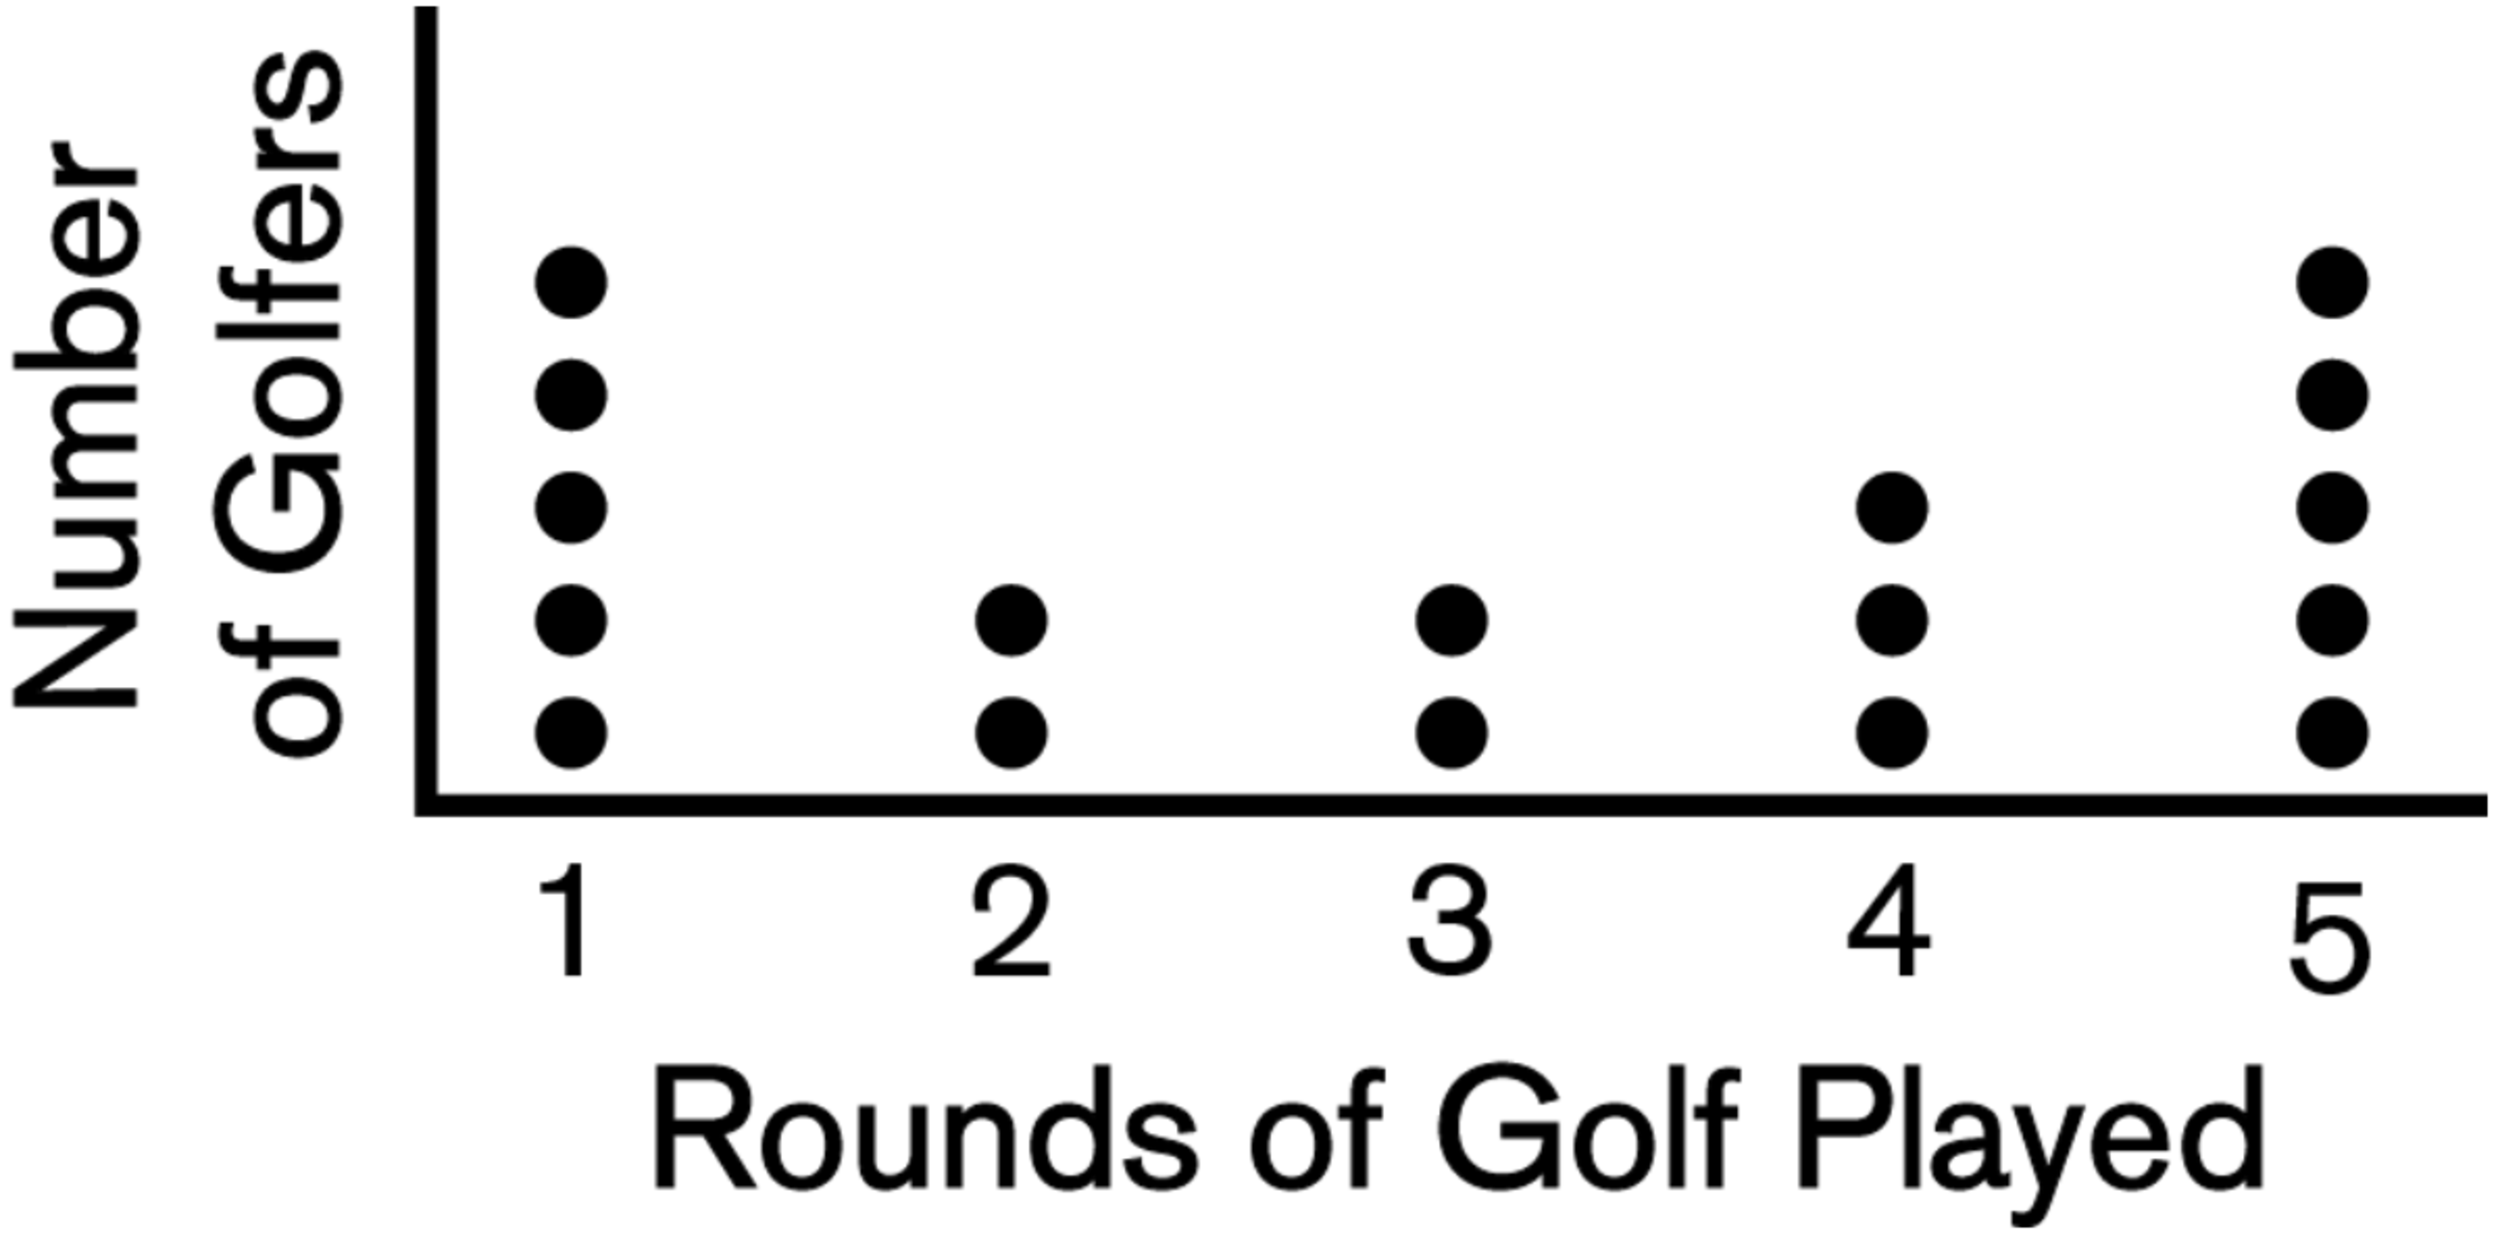
\includegraphics[height=5cm]{sprint-06-figure}
\end{minipagex}


\begin{answer}
\begin{tikzpicture}\node[textbox]{%
    \begin{minipagex}{\dimexpr\textwidth-20pt}
        Reading the data from the graph:
        \begin{align*}
        \frac{5 \cdot 1 + 2 \cdot 2 + 2 \cdot 3 + 3 \cdot 4 + 5 \cdot 5}{5 + 2 + 2 + 3 + 5} = \frac{52}{17} \approx 3
        \end{align*}
        The average number of rounds per golfer is:
        \begin{empheq}[box={\mathbox[colback=white]}]{equation*}
            3 ~\text{rounds}
        \end{empheq}
    \end{minipagex}
    };
\end{tikzpicture}%
\end{answer}
%%%%%%%%%%%%%%%%%%%%%%%%%%%%%%%%%%%%%%%%%%%%%%%%%%%%%%%%%%%%%%%%%%%%%%%%



%%%%%%%%%%%%%%%%%%%%%%%%%%%%%%%%%%%%%%%%%%%%%%%%%%%%%%%%%%%%%%%%%%%%%%%%
\subsection*{7.}
A book company charges a shipping fee of $\$3$ for the first item in a package, $\$2$ for the second item and $\$1$ for each additional item in the package. How many dollars are saved by shipping $10$ items in two packages of five items each, rather than five packages of two items each?

\nopagebreak

\$~\fbox{\phantom{ANSWER}}

\begin{answer}
\begin{tikzpicture}\node[textbox]{%
    \begin{minipagex}{\dimexpr\textwidth-20pt}
        Two packages of five items each:
        \begin{align*}
        2 \times (3 + 2 + 1 + 1 + 1) = 2 \times 8 = 16
        \end{align*}
        Five packages of two items each:
        \begin{align*}
        5 \times (3 + 2) = 5 \times 5 = 25
        \end{align*}
        The difference is $25-16=9$.  The amount saved is:
        \begin{empheq}[box={\mathbox[colback=white]}]{equation*}
            \$~9
        \end{empheq}
    \end{minipagex}
    };
\end{tikzpicture}%
\end{answer}
%%%%%%%%%%%%%%%%%%%%%%%%%%%%%%%%%%%%%%%%%%%%%%%%%%%%%%%%%%%%%%%%%%%%%%%%


%%%%%%%%%%%%%%%%%%%%%%%%%%%%%%%%%%%%%%%%%%%%%%%%%%%%%%%%%%%%%%%%%%%%%%%%
\subsection*{8.}
Algebra exam scores for $27$ students are given in the stem-and-leaf plot shown. What is the arithmetic mean of the median and mode of the given scores?

[Sadly, plot is missing]

\nopagebreak

\fbox{\phantom{ANSWER}}

\begin{answer}
\begin{tikzpicture}\node[textbox]{%
    \begin{minipagex}{\dimexpr\textwidth-20pt}
        The median is $75$. The mode is $71$. 
        \begin{align*}
        \frac{75 + 71}{2} = 73
        \end{align*}
        \begin{empheq}[box={\mathbox[colback=white]}]{equation*}
            73
        \end{empheq}
    \end{minipagex}
    };
\end{tikzpicture}%
\end{answer}
%%%%%%%%%%%%%%%%%%%%%%%%%%%%%%%%%%%%%%%%%%%%%%%%%%%%%%%%%%%%%%%%%%%%%%%%


%%%%%%%%%%%%%%%%%%%%%%%%%%%%%%%%%%%%%%%%%%%%%%%%%%%%%%%%%%%%%%%%%%%%%%%%
\subsection*{9.}
One stamp is randomly selected from a $10$-by-$10$ sheet of $100$ stamps. What is the probability that the stamp selected is not along an outer edge? Express your answer as a common fraction. 

\nopagebreak

\begin{minipage}[b]{\linewidth}
\fbox{\phantom{ANSWER}}\\
\mbox{---------------}\\
\fbox{\phantom{ANSWER}}
\end{minipage}

\begin{answer}
\begin{tikzpicture}\node[textbox]{%
    \begin{minipagex}{\dimexpr\textwidth-20pt}
        Each one of the four edges has $10$ stamps, but the corner stamps belong to two edges, so the total number of edge stamps is $40-4=36$. 
        \begin{align*}
        \frac{100-36}{100} = \frac{64}{100} = \frac{16}{25}
        \end{align*}
        The probability is:
        \begin{empheq}[box={\mathbox[colback=white]}]{equation*}
            \frac{16}{25}
        \end{empheq}
        This problem may be easily generalized to a rectangle. The probability of selecting a stamp not from the outer edge of an $a \times b$ rectangle is:
        \begin{align*}
        \frac{(a-2)(b-2)}{ab}
        \end{align*}
    \end{minipagex}
    };
\end{tikzpicture}%
\end{answer}
%%%%%%%%%%%%%%%%%%%%%%%%%%%%%%%%%%%%%%%%%%%%%%%%%%%%%%%%%%%%%%%%%%%%%%%%


%%%%%%%%%%%%%%%%%%%%%%%%%%%%%%%%%%%%%%%%%%%%%%%%%%%%%%%%%%%%%%%%%%%%%%%%
\subsection*{10.}
The WNBA champions have a twelve-player roster that includes two superstars. If a group of five starting players for this team must include the two superstars, how many different groups of five starting players are there?

\nopagebreak

\fbox{\phantom{ANSWER}}~groups

\begin{answer}
\begin{tikzpicture}\node[textbox]{%
    \begin{minipagex}{\dimexpr\textwidth-20pt}
        Of the $5$ starting players, $2$ are the superstars, so another $3$ must be selected from the remaining $10$ players. 
        \begin{align*}
        \binom{10}{3} = \frac{10!}{7! 3!} = \frac{10 \cdot 9 \cdot 8}{3 \cdot 2} = 5 \cdot 3 \cdot 8 = 120.
        \end{align*}
        \begin{empheq}[box={\mathbox[colback=white]}]{equation*}
            120~\text{groups}
        \end{empheq}
    \end{minipagex}
    };
\end{tikzpicture}%
\end{answer}
%%%%%%%%%%%%%%%%%%%%%%%%%%%%%%%%%%%%%%%%%%%%%%%%%%%%%%%%%%%%%%%%%%%%%%%%


%%%%%%%%%%%%%%%%%%%%%%%%%%%%%%%%%%%%%%%%%%%%%%%%%%%%%%%%%%%%%%%%%%%%%%%%
\subsection*{11.}
Two pencils and one pen cost $\$0.80$, and one pencil and two pens cost $\$1.15$. How many cents would three pencils cost?

\nopagebreak

\fbox{\phantom{ANSWER}}~cents

\begin{answer}
\begin{tikzpicture}\node[textbox]{%
    \begin{minipagex}{\dimexpr\textwidth-20pt}
        Let $p$ denote the price of a pencil and $s$ the price of a pen (`stylus'). We want to solve the linear system for $3p$:
        \begin{align*}
        2 p + 1 s & = 0.80 \\
        1 p + 2 s & = 1.15
        \end{align*}
        Since we want to solve for $3p$, we eliminate $s$ from the system. By subtracting twice the first equation from the second equation, we luckily get our desired solution in a single step:
        \begin{align*}
        (1 -4) p  & = (1.15 - 1.60) \\
         \Rightarrow 3 p  & = 0.45
        \end{align*}
        Three pencils cost:
        \begin{empheq}[box={\mathbox[colback=white]}]{equation*}
            45 ~\text{cents}
        \end{empheq}
    \end{minipagex}
    };
\end{tikzpicture}%
\end{answer}
%%%%%%%%%%%%%%%%%%%%%%%%%%%%%%%%%%%%%%%%%%%%%%%%%%%%%%%%%%%%%%%%%%%%%%%%


%%%%%%%%%%%%%%%%%%%%%%%%%%%%%%%%%%%%%%%%%%%%%%%%%%%%%%%%%%%%%%%%%%%%%%%%
\subsection*{12.}
There are $8$ furlongs in a mile. There are $2$ weeks in a fortnight. The British cavalry traveled $2800$ furlongs in a fortnight. How many miles per day did the cavalry average?

\nopagebreak

\fbox{\phantom{ANSWER}}~miles per day

\begin{answer}
\begin{tikzpicture}\node[textbox]{%
    \begin{minipagex}{\dimexpr\textwidth-20pt}
        To convert a fortnight into days, divide by $2 \times 7$ (two weeks, seven days per week). To convert a furlong to a mile, divide by $8$.
        \begin{align*}
        \frac{2800}{2 \times 7 \times 8} = \frac{14 \times 100}{7 \times 8} =  \frac{100}{4} = 25
        \end{align*}
        The average distance is:
        \begin{empheq}[box={\mathbox[colback=white]}]{equation*}
            25~\text{miles per day}
        \end{empheq}
    \end{minipagex}
    };
\end{tikzpicture}%
\end{answer}
%%%%%%%%%%%%%%%%%%%%%%%%%%%%%%%%%%%%%%%%%%%%%%%%%%%%%%%%%%%%%%%%%%%%%%%%


%%%%%%%%%%%%%%%%%%%%%%%%%%%%%%%%%%%%%%%%%%%%%%%%%%%%%%%%%%%%%%%%%%%%%%%%
\subsection*{13.}
Two cubes have edge lengths of $6$ inches and $12$ inches. What is the ratio of the surface area of the smaller cube to the surface area of the large cube? Express your answer as a common fraction. 

\nopagebreak

\begin{minipage}[b]{\linewidth}
\fbox{\phantom{ANSWER}}\\
\mbox{---------------}\\
\fbox{\phantom{ANSWER}}
\end{minipage}

\begin{answer}
\begin{tikzpicture}\node[textbox]{%
    \begin{minipagex}{\dimexpr\textwidth-20pt}
        Each cube has $6$ faces, so the surface area of a cubes with edge $a$ is $6a^{2}$. The ratio of the smaller to the larger cube is therefore:
        \begin{align*}
        \frac{6 \cdot 6^2}{6 \cdot 12^2} = \left(\frac{6}{12}\right)^2 = \left(\frac{1}{2}\right)^2 = \frac{1}{4}
        \end{align*}
        The ratio is:
        \begin{empheq}[box={\mathbox[colback=white]}]{equation*}
            \frac{1}{4}
        \end{empheq}
    \end{minipagex}
    };
\end{tikzpicture}%
\end{answer}
%%%%%%%%%%%%%%%%%%%%%%%%%%%%%%%%%%%%%%%%%%%%%%%%%%%%%%%%%%%%%%%%%%%%%%%%


%%%%%%%%%%%%%%%%%%%%%%%%%%%%%%%%%%%%%%%%%%%%%%%%%%%%%%%%%%%%%%%%%%%%%%%%
\subsection*{14.}
Phil Lanthropist won a great deal of money in a contest. He gave $20\%$ of his winnings to his parents, $25\%$ of the remaining money to his children, and the remaining $\$900,000$ to his favorite charity. What was the total number of dollars that Phil won?

\nopagebreak

\$~\fbox{\phantom{ANSWER}}

\begin{answer}
\begin{tikzpicture}\node[textbox]{%
    \begin{minipagex}{\dimexpr\textwidth-20pt}
        Let $w$ denote the winnings. After giving to this parents, there remain $0.8w$. After giving to the children, only $0.75$ of that remains to be given to the charity. Thus
        \begin{align*}
        0.75 \times 0.8 \times w & = 900,000 \\
        \Rightarrow w & = \frac{900,000 \times 1000}{75 \times 8} \\
          & = \frac{9 \times 1,000,000}{6} \\
          & = 1,500,000
        \end{align*}
        The winnings were:
        \begin{empheq}[box={\mathbox[colback=white]}]{equation*}
            \$1~500~000
        \end{empheq}
    \end{minipagex}
    };
\end{tikzpicture}%
\end{answer}
%%%%%%%%%%%%%%%%%%%%%%%%%%%%%%%%%%%%%%%%%%%%%%%%%%%%%%%%%%%%%%%%%%%%%%%%


%%%%%%%%%%%%%%%%%%%%%%%%%%%%%%%%%%%%%%%%%%%%%%%%%%%%%%%%%%%%%%%%%%%%%%%%
\subsection*{15.}
Two circles with spinners at their centers are divided into three equal regions, as shown. When both spinners are spun, what is the probability that the product of the two values is negative? Express your answer as a common fraction.

\nopagebreak

\begin{minipage}[b]{\linewidth}
\fbox{\phantom{ANSWER}}\\
\mbox{---------------}\\
\fbox{\phantom{ANSWER}}
\end{minipage}

\begin{minipagex}[b]{\linewidth}
\centering
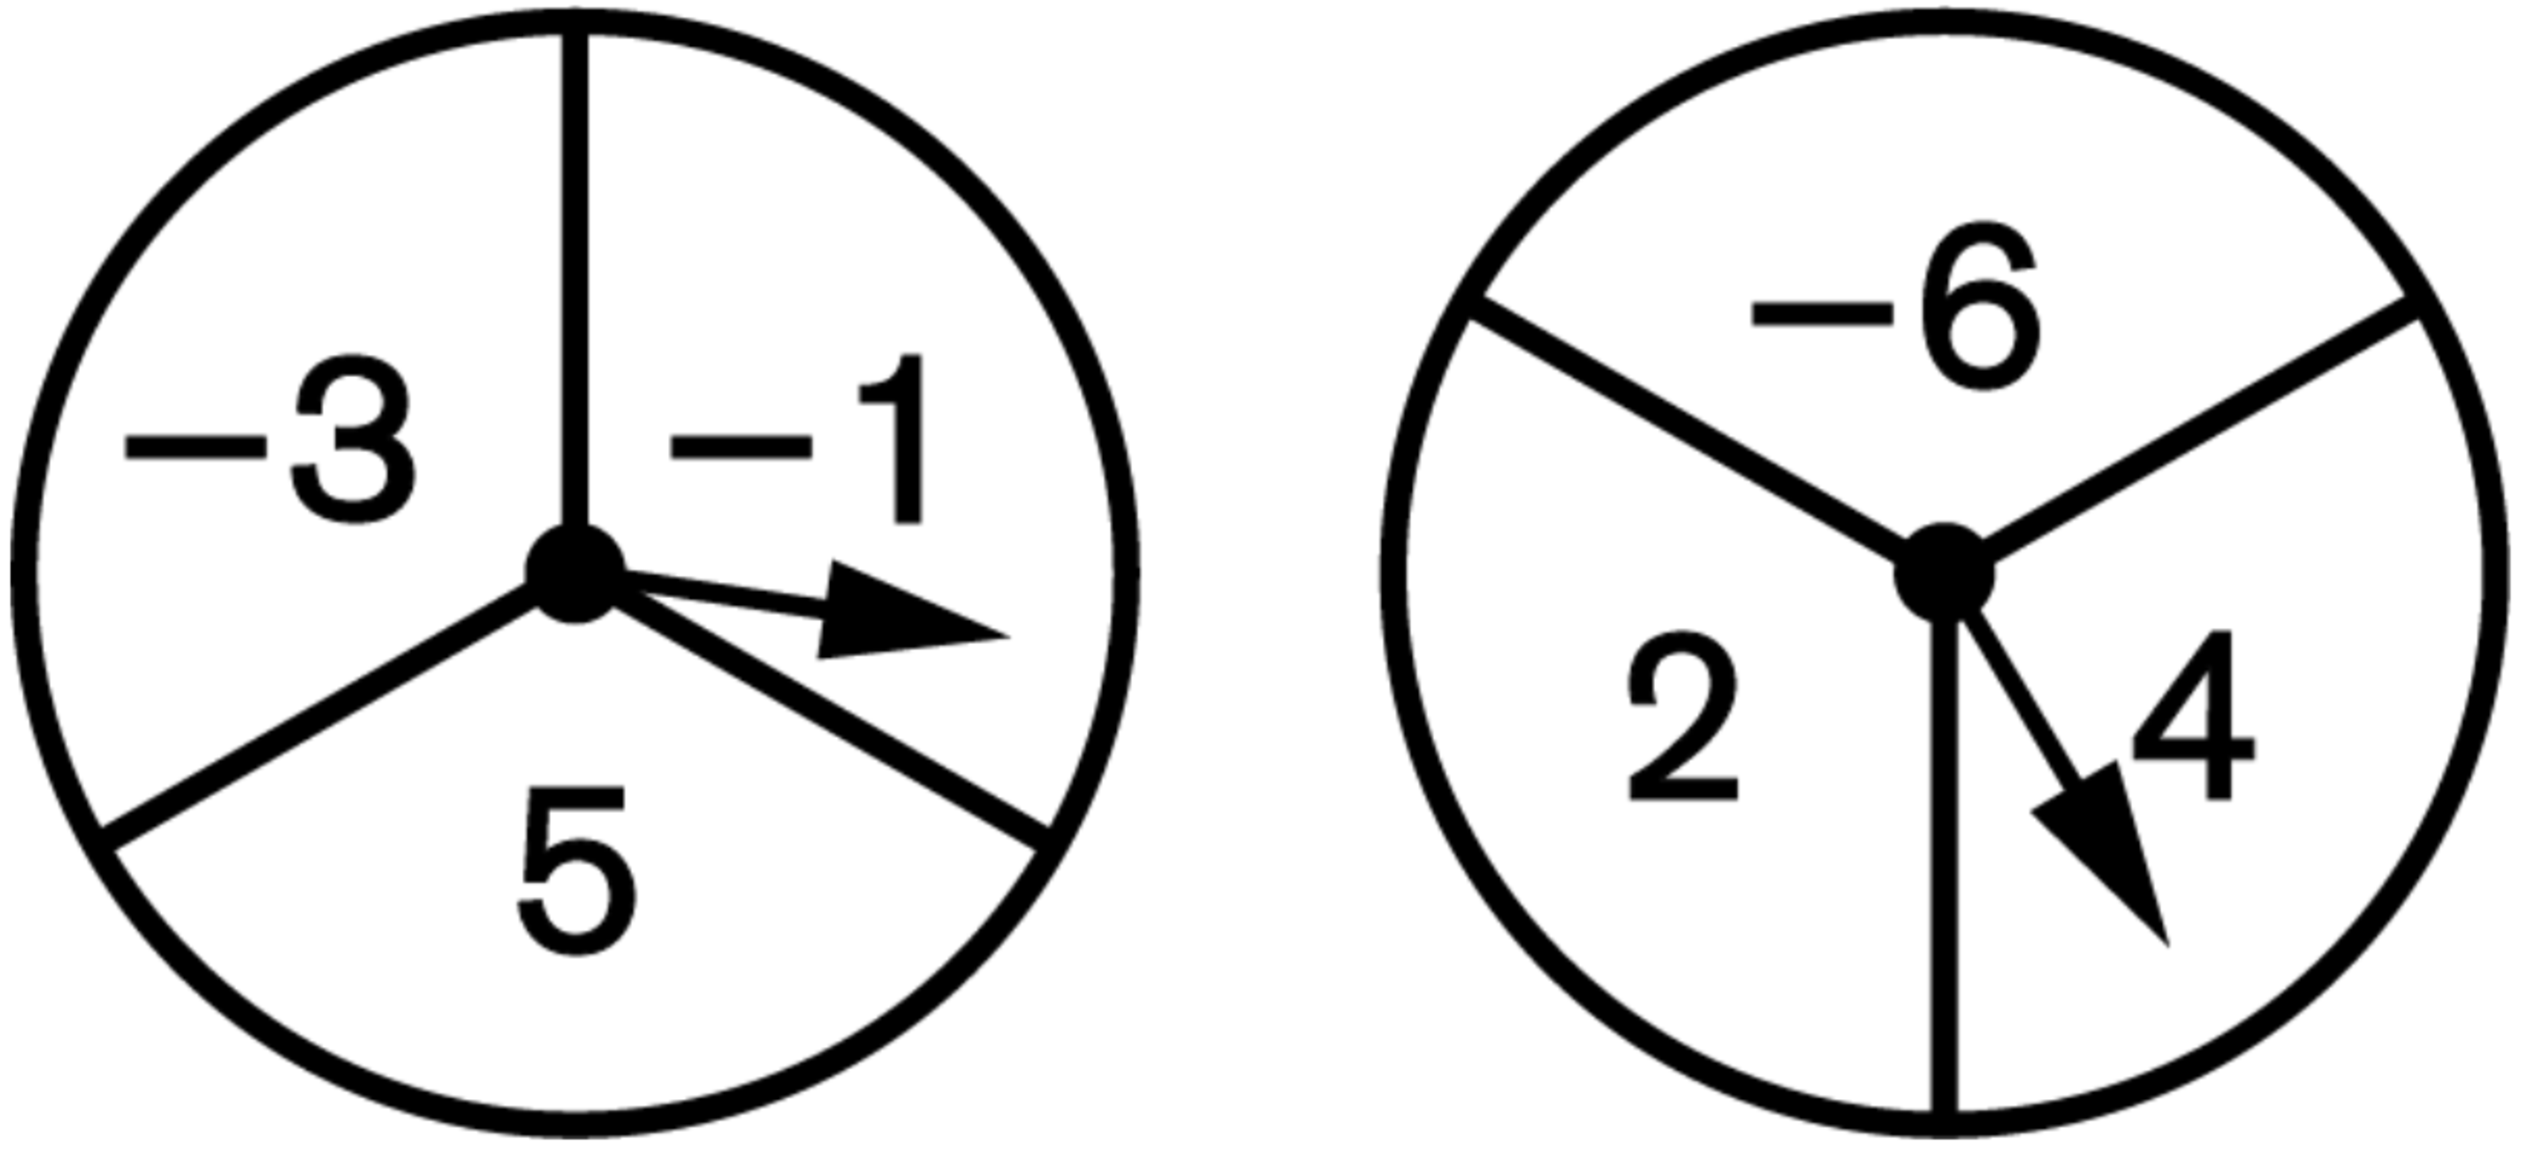
\includegraphics[height=3cm]{sprint-15-figure}
\end{minipagex}

\begin{answer}
\begin{tikzpicture}\node[textbox]{%
    \begin{minipagex}{\dimexpr\textwidth-20pt}
        There are two ways to obtain a negative product: Either draw a negative integer from the first spinner (with probability $2/3$) and a positive integer from the second spinner (with probability $2/3$). Or draw a positive integer from the first spinner (with probability $1/3$) and a negative integer from the second spinner (with probability $1/3$). Thus,
        \begin{align*}
        \left(\frac{2}{3} \cdot \frac{2}{3}\right) + \left(\frac{1}{3} \cdot \frac{1}{3}\right) 
        = \frac{2 \cdot 2 + 1 \cdot 1}{3 \cdot 3} = \frac{5}{9}
        \end{align*}
        The probability is:
        \begin{empheq}[box={\mathbox[colback=white]}]{equation*}
            \frac{5}{9}
        \end{empheq}
    \end{minipagex}
    };
\end{tikzpicture}%
\end{answer}
%%%%%%%%%%%%%%%%%%%%%%%%%%%%%%%%%%%%%%%%%%%%%%%%%%%%%%%%%%%%%%%%%%%%%%%%


%%%%%%%%%%%%%%%%%%%%%%%%%%%%%%%%%%%%%%%%%%%%%%%%%%%%%%%%%%%%%%%%%%%%%%%%
\subsection*{16.}
Cheldelin Middle School has $12$ doors to enter or leave the building. In how many ways is it possible to enter the building by one door and leave the building by a different door?

\nopagebreak

\fbox{\phantom{ANSWER}}~ways

\begin{answer}
\begin{tikzpicture}\node[textbox]{%
    \begin{minipagex}{\dimexpr\textwidth-20pt}
        To get a handle on the problem, consider simple cases. For instance, $3$ doors labeled A, B, C. In this case,there are $6$ ways: AB, AC, BA, BC, CA, CB. Other example: $4$ doors labeled A, B, C, D. In this case, there are $12$ ways: AB, AC, AD, BA, BC, BD, CA, CB, CD, DA, DB, DC. Clearly the formula for $n$ doors is $n(n-1)$: There are $n$ doors to choose from on the way in, but only $n-1$ doors left to choose from on the way out. And thus,
        \begin{align*}
        12 \times 11 = 132
        \end{align*}
        \begin{empheq}[box={\mathbox[colback=white]}]{equation*}
            132~\text{ways}
        \end{empheq}
    \end{minipagex}
    };
\end{tikzpicture}%
\end{answer}
%%%%%%%%%%%%%%%%%%%%%%%%%%%%%%%%%%%%%%%%%%%%%%%%%%%%%%%%%%%%%%%%%%%%%%%%


%%%%%%%%%%%%%%%%%%%%%%%%%%%%%%%%%%%%%%%%%%%%%%%%%%%%%%%%%%%%%%%%%%%%%%%%
\subsection*{17.}
Sue is four times as old as Tom is now, and she is $\dfrac{8}{3}$ as old as Tom will be in $7$ years. How many years old was Tom three years ago?

\nopagebreak

\fbox{\phantom{ANSWER}}~years old

\begin{answer}
\begin{tikzpicture}\node[textbox]{%
    \begin{minipagex}{\dimexpr\textwidth-20pt}
        Let $s$ and $t$ denote the ages of Sue and Tom now. We want to calculate $t-3$. The question is equivalent to the linear system in the two unknowns $s$ and $t$:
        \begin{align*}
        s & = 4 t \\
        s & = \frac{8}{3} \left(t + 7\right)
        \end{align*}
        By substituting $4t$ into $s$ and multiplying by $3$ to eliminate the fraction, we get
        \begin{align*}
        3 \cdot 4 t & = 8 (t + 7) \\
        \Rightarrow 
           (12-8) t & = 7 \cdot 8 \\
        \Rightarrow t 
                    & = \frac{7 \cdot 8}{4} = 7 \cdot 2 \\
        \Rightarrow t - 3 
                    & = 14 - 3 = 11
        \end{align*}
        \begin{empheq}[box={\mathbox[colback=white]}]{equation*}
            11~\text{years old}
        \end{empheq}
    \end{minipagex}
    };
\end{tikzpicture}%
\end{answer}
%%%%%%%%%%%%%%%%%%%%%%%%%%%%%%%%%%%%%%%%%%%%%%%%%%%%%%%%%%%%%%%%%%%%%%%%


%%%%%%%%%%%%%%%%%%%%%%%%%%%%%%%%%%%%%%%%%%%%%%%%%%%%%%%%%%%%%%%%%%%%%%%%
\subsection*{18.}
By hitting a target, Juanita can score $16$, $17$, $23$, $26$, $29$ or $40$ points with each arrow she shoots. What is the fewest arrows she can shoot to score exactly $100$ points?

\nopagebreak

\fbox{\phantom{ANSWER}}~arrows

\begin{answer}
\begin{tikzpicture}\node[textbox]{%
    \begin{minipagex}{\dimexpr\textwidth-20pt}
        We first note that the minimum number of arrows needed is $4$. This follows from:
        \begin{align*}
        & 40 + 40 + 40 = 120 > 100 \\
        & 40 + 40 + 29 = 109 > 100 \\
        & 40 + 40 + 26 = 106 > 100 \\
        & 40 + 40 + 23 = 103 > 100 \\
        & 40 + 40 + 17 = 97  < 100
        \end{align*}
        We will solve the problem by trial and error, looking to reduce the number of trials. To minimize the number of arrows, we would like to use large scores. For instance, hitting $40$ twice takes us to $80$. Unfortunately, there is no way to hit $20$. We also note that $17+23=40$, so it is never optimal to target $17$ and $23$ since the same score can be obtained with one arrow on $40$. We also note that $17+17=34$, which ends in a $4$: we have $16$ and $26$, can we get to $60$? Yes we can! We can hit $100$ with two arrows on $17$, one arrow on $26$, and one arrow on $40$, for a total of four arrows:
        \begin{align*}
        2 \times (17) + 1 \times (26) + 1 \times (40)
        \end{align*}
        \begin{empheq}[box={\mathbox[colback=white]}]{equation*}
            4 ~\text{arrows}
        \end{empheq}
        We had also found that four arrows on $17$ and two arrows on $16$ gets to $100$, but that's a total of six arrows, so not as good. 
    \end{minipagex}
    };
\end{tikzpicture}%
\end{answer}
%%%%%%%%%%%%%%%%%%%%%%%%%%%%%%%%%%%%%%%%%%%%%%%%%%%%%%%%%%%%%%%%%%%%%%%%


%%%%%%%%%%%%%%%%%%%%%%%%%%%%%%%%%%%%%%%%%%%%%%%%%%%%%%%%%%%%%%%%%%%%%%%%
\subsection*{19.}
Twenty students bought tickets for a school party. All of the money received for these $20$ tickets was used to purchase beverages. Then, an additional $10$ students bought tickets. Rather than use this additional money to buy more refreshments, all $30$ students received a $\$3.00$ refund. How many dollars were used to buy beverages?

\nopagebreak

\fbox{\phantom{ANSWER}}

\begin{answer}
\begin{tikzpicture}\node[textbox]{%
    \begin{minipagex}{\dimexpr\textwidth-20pt}
        Let $p$ denote the price of a ticket. The total money contributed towards beverages is $20p$. The money contributed by the additional students, $10p$, is refunded to all $30$ students, with each receiving $\$3$, so we have
        \begin{align*}
        \frac{10p}{30} & = 3 \\
        \Rightarrow p & = 9 \\
        \Rightarrow 20p & = 20 \times 9 = 180
        \end{align*}
        The cost of beverages:
        \begin{empheq}[box={\mathbox[colback=white]}]{equation*}
            \$~180
        \end{empheq}
    \end{minipagex}
    };
\end{tikzpicture}%
\end{answer}
%%%%%%%%%%%%%%%%%%%%%%%%%%%%%%%%%%%%%%%%%%%%%%%%%%%%%%%%%%%%%%%%%%%%%%%%


%%%%%%%%%%%%%%%%%%%%%%%%%%%%%%%%%%%%%%%%%%%%%%%%%%%%%%%%%%%%%%%%%%%%%%%%
\subsection*{20.}
A jar contains $10$ red, $7$ blue, and $5$ yellow marbles. What is the least number of blue marbles that must be added to the jar so that the probability of randomly selecting a blue marble is greater than $\dfrac{1}{2}$?

\nopagebreak

\fbox{\phantom{ANSWER}}~blue marbles

\begin{answer}
\begin{tikzpicture}\node[textbox]{%
    \begin{minipagex}{\dimexpr\textwidth-20pt}
        The number of blue marbles must be greater than the number of non-blue marbles:
        \begin{align*}
        7 + x & > 10 + 5 \\
        \Rightarrow x & > 8
        \end{align*}
        The smallest number of blue marbles to be added:
        \begin{empheq}[box={\mathbox[colback=white]}]{equation*}
            9
        \end{empheq}
    \end{minipagex}
    };
\end{tikzpicture}%
\end{answer}
%%%%%%%%%%%%%%%%%%%%%%%%%%%%%%%%%%%%%%%%%%%%%%%%%%%%%%%%%%%%%%%%%%%%%%%%


%%%%%%%%%%%%%%%%%%%%%%%%%%%%%%%%%%%%%%%%%%%%%%%%%%%%%%%%%%%%%%%%%%%%%%%%
\subsection*{21.}
Terry is purchasing a bike that is on sale for $40\%$ off the original price. After a coupon is applied that reduces the sale price by $20\%$, Terry's final  cost for the bike is $\$168$. What was the original price of the bike Terry is purchasing?

\nopagebreak

\$~\fbox{\phantom{ANSWER}}

\begin{answer}
\begin{tikzpicture}\node[textbox]{%
    \begin{minipagex}{\dimexpr\textwidth-20pt}
        Two discounts are applied to the original price $p$. Terry pays $80\%$ of $60\%$ of the original price $p$, so that
        \begin{align*}
        0.8 \times 0.6 \times p & = 168 \\
        \Rightarrow 
        p & = \frac{168 \times 100}{2^3 \times 3 \times 2} \\
          & = \frac{21}{3}  \times \frac{100}{2} \\
          & = 350
        \end{align*}
        The original price is:
        \begin{empheq}[box={\mathbox[colback=white]}]{equation*}
            350
        \end{empheq}
    \end{minipagex}
    };
\end{tikzpicture}%
\end{answer}
%%%%%%%%%%%%%%%%%%%%%%%%%%%%%%%%%%%%%%%%%%%%%%%%%%%%%%%%%%%%%%%%%%%%%%%%




%%%%%%%%%%%%%%%%%%%%%%%%%%%%%%%%%%%%%%%%%%%%%%%%%%%%%%%%%%%%%%%%%%%%%%%%
\subsection*{22.}
Two cylindrical cans have the same volume. The height of one can is triple the height of the other. If the radius of the narrower can is $12$ units, how many units are in the length of the radius of the wider can? Express your answer in simplest radical form. 

\begin{minipagex}[b]{\linewidth}
\centering
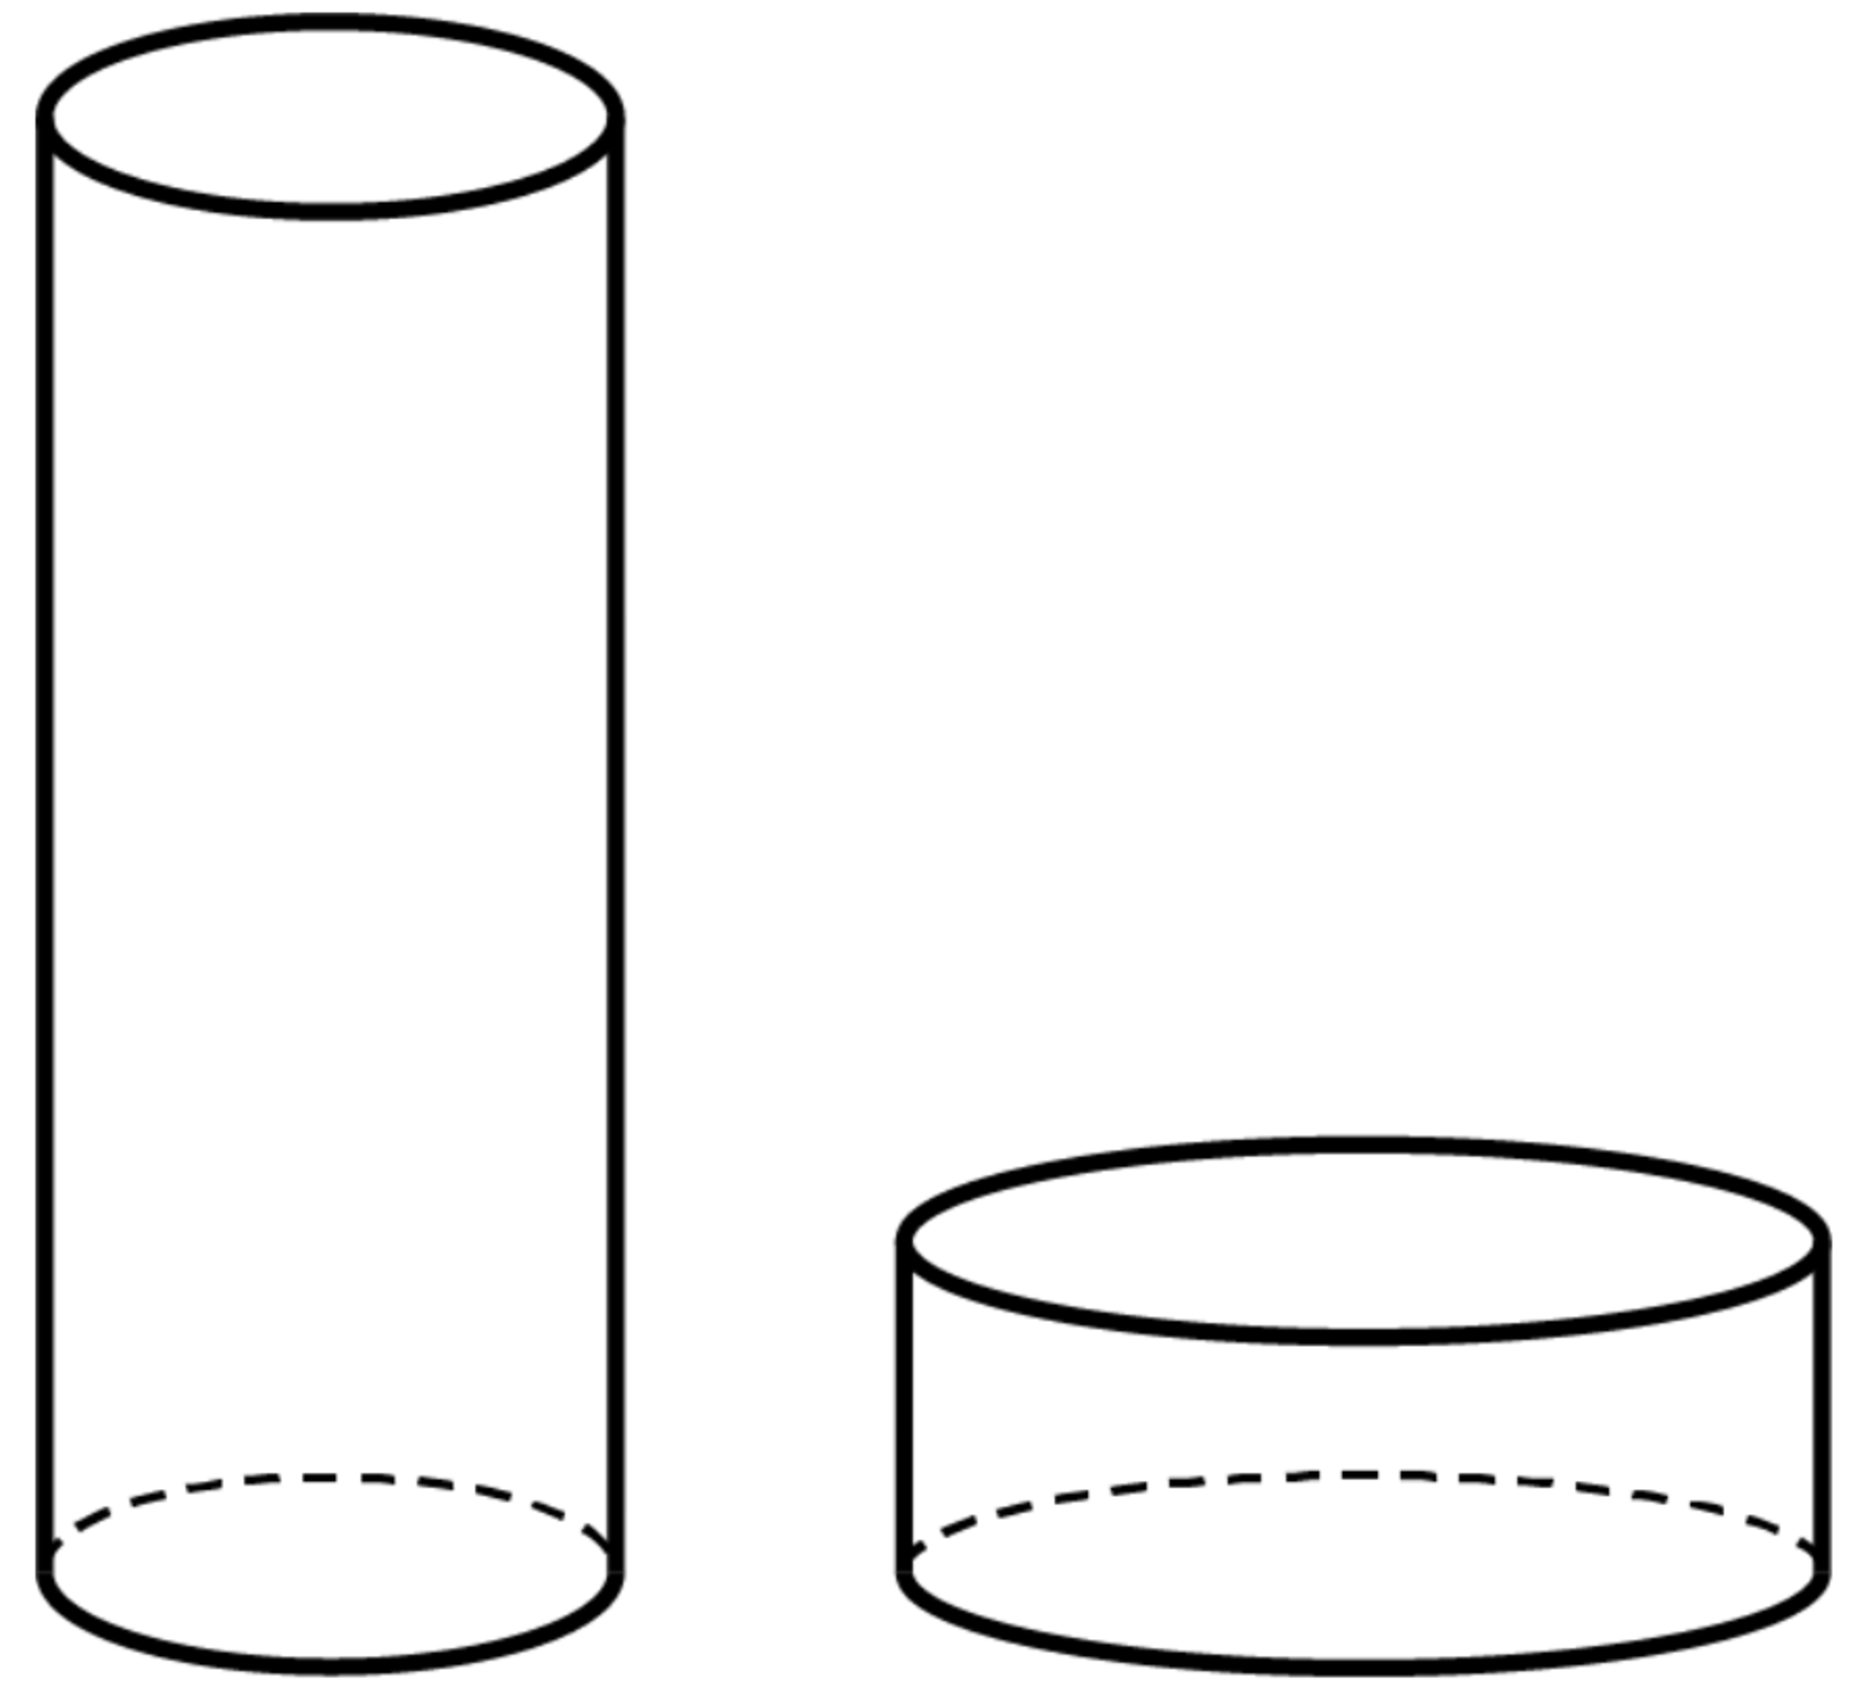
\includegraphics[height=3cm]{sprint-22-figure}
\end{minipagex}

\nopagebreak

\fbox{\phantom{ANSWER}}$\sqrt{\fbox{\phantom{ANSWER}}}$

\begin{answer}
\begin{tikzpicture}\node[textbox]{%
    \begin{minipagex}{\dimexpr\textwidth-20pt}
        The volume of a cylinder is equal to the surface area of the circular face multiplied by the height of the cylinder. 
        Let $(r, H)$ done the radius and height of the taller cylinder and $(R, h)$ the radius and height of the other cylinder. Since the volumes are equal, we may write:
        \begin{align*}
        \pi r^2 \times H & = \pi R^2 \times h \\
        R^2 & = r^2 \times \frac{H}{h}
        \end{align*}
        Since $H=3h$, we get:
        \begin{align*}
        R = r\sqrt{3} = 12\sqrt{3}
        \end{align*}
        \begin{empheq}[box={\mathbox[colback=white]}]{equation*}
            12\sqrt{3}
        \end{empheq}
    \end{minipagex}
    };
\end{tikzpicture}%
\end{answer}
%%%%%%%%%%%%%%%%%%%%%%%%%%%%%%%%%%%%%%%%%%%%%%%%%%%%%%%%%%%%%%%%%%%%%%%%


%%%%%%%%%%%%%%%%%%%%%%%%%%%%%%%%%%%%%%%%%%%%%%%%%%%%%%%%%%%%%%%%%%%%%%%%
\subsection*{23.}
How many terms of the arithmetic sequence $88$, $85$, $82$, $\ldots$ appear before the number $-17$ appears?

\nopagebreak

\fbox{\phantom{ANSWER}}~terms

\begin{answer}
\begin{tikzpicture}\node[textbox]{%
    \begin{minipagex}{\dimexpr\textwidth-20pt}
        Starting from $88$, subtract $3$ repeatedly until you reach $-14$ (the number before $-17$). If $k$ denotes the number of steps needed to reach $-14$, then $k+1$ is the number of terms in the sequence. Thus,
        \begin{align*}
        88 - 3k & = -14 \\
        \Rightarrow k & = \frac{102}{3} = 34 \\
        k + 1 & = 35
        \end{align*}
        \begin{empheq}[box={\mathbox[colback=white]}]{equation*}
            35 ~\text{terms}
        \end{empheq}
    \end{minipagex}
    };
\end{tikzpicture}%
\end{answer}
%%%%%%%%%%%%%%%%%%%%%%%%%%%%%%%%%%%%%%%%%%%%%%%%%%%%%%%%%%%%%%%%%%%%%%%%


%%%%%%%%%%%%%%%%%%%%%%%%%%%%%%%%%%%%%%%%%%%%%%%%%%%%%%%%%%%%%%%%%%%%%%%%
\subsection*{24.}
In the chess club, there are $15$ eight graders, $6$ of whom wear glasses. Nine students in the chess club wear glasses. Eight students in the chess club are neither eighth graders nor wear glasses. How many people are in the chess club? 

\nopagebreak

\fbox{\phantom{ANSWER}}~people

\begin{answer}
\begin{tikzpicture}\node[textbox]{%
    \begin{minipagex}{\dimexpr\textwidth-20pt}
        One approach is to construct the set of chess players from the available information. Let $8$ denote an eighth grader and $0$ denote a non-eighth grader. Let $G$ denote glasses. Adding members from left to right based on the above description yields:
        \begin{align*}
        8, 8, 8, 8, 8, 8, 8, 8, 8, 8G, 8G, 8G, 8G, 8G, 8G, 0G, 0G, 0G, 0, 0, 0, 0, 0, 0, 0, 0
        \end{align*}
        for a total of $15 + 3 + 8 = 26$ people. 
        \begin{empheq}[box={\mathbox[colback=white]}]{equation*}
            26~\text{people}
        \end{empheq}
    \end{minipagex}
    };
\end{tikzpicture}%
\end{answer}
%%%%%%%%%%%%%%%%%%%%%%%%%%%%%%%%%%%%%%%%%%%%%%%%%%%%%%%%%%%%%%%%%%%%%%%%


%%%%%%%%%%%%%%%%%%%%%%%%%%%%%%%%%%%%%%%%%%%%%%%%%%%%%%%%%%%%%%%%%%%%%%%%
\subsection*{25.}
In a sequence, each term after the first is four more than three times the previous term. The fifth term of this sequence is $403$. What is the first term?

\nopagebreak

\fbox{\phantom{ANSWER}}

\begin{answer}
\begin{tikzpicture}\node[textbox]{%
    \begin{minipagex}{\dimexpr\textwidth-20pt}
        It is convenient to start from the fifth term and take four steps back to the first term, by subtracting $4$ and dividing by $3$ at each step. Starting from $403$, we reach $3$ after $4$ steps.
        \begin{align*}
        \frac{403 - 4}{3} & = 133 \\
        \frac{133 - 4}{3} & = 43 \\
        \frac{43 - 4}{3} & = 13 \\
        \frac{13 - 4}{3} & = 3 
        \end{align*}
        The first term is:
        \begin{empheq}[box={\mathbox[colback=white]}]{equation*}
            3
        \end{empheq}
    \end{minipagex}
    };
\end{tikzpicture}%
\end{answer}
%%%%%%%%%%%%%%%%%%%%%%%%%%%%%%%%%%%%%%%%%%%%%%%%%%%%%%%%%%%%%%%%%%%%%%%%


%%%%%%%%%%%%%%%%%%%%%%%%%%%%%%%%%%%%%%%%%%%%%%%%%%%%%%%%%%%%%%%%%%%%%%%%
\subsection*{26.}
The average value of nine consecutive integers is $13$. What is the sum of the smallest and largest of these integers?

\nopagebreak

\fbox{\phantom{ANSWER}}

\begin{answer}
\begin{tikzpicture}\node[textbox]{%
    \begin{minipagex}{\dimexpr\textwidth-20pt}
        The average value of nine consecutive integers $n_{1}$, $\ldots$, $n_{9}$ is
        \begin{align*}
        \frac{n_{1} + n_{2} + \ldots + n_{9}}{9} = 13 \\
        \Rightarrow 
        n_{1} + n_{2} + \ldots + n_{9} = 117
        \end{align*}
        The sum of the first $9$ integers is $(9 \times 10)/2=45$. The sum of the first $18$ integers is $(18 \times 19)/2=171$. Since $171-45=126>117$, the sum we are looking for starts below $10$. A good guess is $9$. This can be seen without recalculating the sum:
        \begin{alignat*}{3}
            &10 + 11 &&+ \ldots + 17 + 18 &&= 126 \\
        9 + &10 + 11 &&+ \ldots + 17      &&= 126 -18 + 9 = 117 
        \end{alignat*}
        The sum of the smallest and largest integers are then:
        \begin{align*}
        9 + 17 = 26 
        \end{align*}
        \begin{empheq}[box={\mathbox[colback=white]}]{equation*}
            26
        \end{empheq}
    \end{minipagex}
    };
\end{tikzpicture}%
\end{answer}
%%%%%%%%%%%%%%%%%%%%%%%%%%%%%%%%%%%%%%%%%%%%%%%%%%%%%%%%%%%%%%%%%%%%%%%%


%%%%%%%%%%%%%%%%%%%%%%%%%%%%%%%%%%%%%%%%%%%%%%%%%%%%%%%%%%%%%%%%%%%%%%%%
\subsection*{27.}
A $24$-foot by $72$-foot rectangular dance floor is completely tiled with $1$-foot by $1$-foot square tiles. Two opposite corners of the dance floor are connected by a diagonal. This diagonal passes through the interior of exactly how many tiles?

\nopagebreak

\fbox{\phantom{ANSWER}}~tiles

\begin{answer}
\begin{tikzpicture}\node[textbox]{%
    \begin{minipagex}{\dimexpr\textwidth-20pt}
        Consider simple cases. With a $2$-by-$2$ pattern, the diagonal passes through $2$ tiles. If this pattern is doubled to $4$-by-$4$, the diagonal passes through $4$ tiles and, in general, in a $2n$-by-$2n$ pattern the diagonal passes through $2n$ tiles. In words, multiplying the sides by a common factor results in multiplying the number of tiles passed by that same factor. This property is in fact general (and is easy to see by example). With a $3$-by-$1$ pattern, the diagonal passes through all $3$ tiles, and therefore with a $3n$-by-$1n$ pattern, the diagonal passes through $3n$ tiles. Since $72 = 3 \times 24$, the $24$-by-$72$ pattern can be reduced to the $1$-by-$3$ pattern, where the diagonal passes through $3$ tiles. The total number of squares is then obtained by multiplying the number of tiles by $24$:
        \begin{align*}
        24 \times 3 = 72
        \end{align*}
        \begin{empheq}[box={\mathbox[colback=white]}]{equation*}
            72~\text{tiles}
        \end{empheq}
    \end{minipagex}
    };
\end{tikzpicture}%
\end{answer}
%%%%%%%%%%%%%%%%%%%%%%%%%%%%%%%%%%%%%%%%%%%%%%%%%%%%%%%%%%%%%%%%%%%%%%%%


%%%%%%%%%%%%%%%%%%%%%%%%%%%%%%%%%%%%%%%%%%%%%%%%%%%%%%%%%%%%%%%%%%%%%%%%
\subsection*{28.}
Starting at the M and moving left, right, up, down to an adjoining letter, how many distinct paths can be followed to spell the word MATH?

\nopagebreak

\fbox{\phantom{ANSWER}}~paths

\begin{minipagex}[b]{\linewidth}
\centering
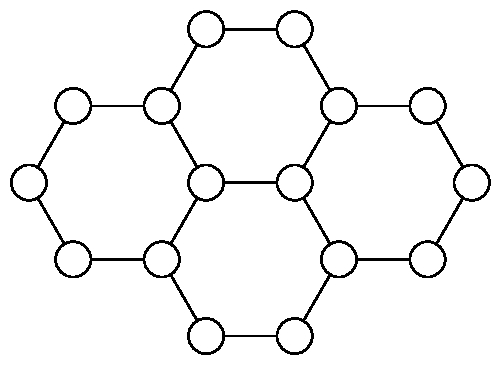
\includegraphics[height=4cm]{sprint-28-figure}
\end{minipagex}

\begin{answer}
\begin{tikzpicture}\node[textbox]{%
    \begin{minipagex}{\dimexpr\textwidth-20pt}
        There is only one starting point, M. By symmetry, we can focus on a quarter of the figure, say North-East, and multiply by $4$. Let E denote a step to the East and N a step to the North. Starting from M, there are two possible directions: East or North. We find: EEE, EEN, ENE, ENN ($4$ paths to the East), and NEE, NEN, NNE, NNN ($4$ paths to the North). If we count both EEE and NNN we will be double-counting, so we drop one of them. Putting it together,
        \begin{align*}
        4 \times (4+4-1) = 28
        \end{align*}
        \begin{empheq}[box={\mathbox[colback=white]}]{equation*}
            28~\text{paths}
        \end{empheq}
    \end{minipagex}
    };
\end{tikzpicture}%
\end{answer}
%%%%%%%%%%%%%%%%%%%%%%%%%%%%%%%%%%%%%%%%%%%%%%%%%%%%%%%%%%%%%%%%%%%%%%%%


%%%%%%%%%%%%%%%%%%%%%%%%%%%%%%%%%%%%%%%%%%%%%%%%%%%%%%%%%%%%%%%%%%%%%%%%
\subsection*{29.}
Given that $3^3 \times 9^3 \times 27^3 \times 81^3 = 9^x$, what is the value of $x$?

\nopagebreak

\fbox{\phantom{ANSWER}}

\begin{answer}
\begin{tikzpicture}\node[textbox]{%
    \begin{minipagex}{\dimexpr\textwidth-20pt}
        \begin{alignat*}{4}
        & ~~~~~~3^3 &&\times 9^3 &&\times ~~~27^3 &&\times ~~~81^3 \\
        & = 3 \times 9^1 &&\times 9^3 &&\times (3\times 9)^3 &&\times (9 \times 9)^3 \\
        & = 3 \times 9^1 &&\times 9^3 &&\times 3 \times 9^1 \times 9^3~~~~~ &&\times 9^6
        \end{alignat*}
        Adding the exponents on $9$, in the order above, yields:
        \begin{align*}
        1/2 + 1 + 3 + 1/2 + 1 + 3 + 6 = 15
        \end{align*}
        \begin{empheq}[box={\mathbox[colback=white]}]{equation*}
            15
        \end{empheq}
    \end{minipagex}
    };
\end{tikzpicture}%
\end{answer}
%%%%%%%%%%%%%%%%%%%%%%%%%%%%%%%%%%%%%%%%%%%%%%%%%%%%%%%%%%%%%%%%%%%%%%%%


%%%%%%%%%%%%%%%%%%%%%%%%%%%%%%%%%%%%%%%%%%%%%%%%%%%%%%%%%%%%%%%%%%%%%%%%
\subsection*{30.}
Camy made a list of all distinct five-digit positive even integers whose digits are $1$, $3$, $4$, $5$, and $9$. What is the sum of the integers on Camy's list?

\nopagebreak

\fbox{\phantom{ANSWER}}

\begin{answer}
\begin{tikzpicture}\node[textbox]{%
    \begin{minipagex}{\dimexpr\textwidth-20pt}
        Writing out all the possible integers is not practical, so we look for a pattern. First, note that since the integers must be even, they must all have $4$ in the unit column. Thus the sum of all the units will contribute $4n$ to the total sum, where $n$ is the number of integers in the list. Secondly, note that every digit will appear the same number of times in the ten, hundred, thousand, and ten-thousand columns (because there are no restrictions on where the digits can be used other than placing the $4$ in the unit column). Thus, the sum of these columns will contribute $(10,000+1000+100+10)s=11110s$, where $s$ is the sum of the digits in one column. The total sum is therefore $11110s+4n$, where $n$ and $s$ are to be determined. 
        
        The number of five-digit integers ending in $4$ is the same as the number of four-digit integers created with $1$, $3$, $5$, and $9$, or $24$ distinct integers:
        \begin{align*}
        n = 4! = 4 \times 3 \times 2 = 24
        \end{align*}
        Each of the four integers $1$, $3$, $5$, $9$ will appear the same number of times in a given column, or $24/4=6$ times. Thus, the sum is
        \begin{align*}
        s = 6 \times (1+3+5+9) = 6 \times 18 = 108
        \end{align*}
        Putting it together:
        \begin{align*}
        11110s + 4n = 11110 \times 108 + 4 \times 24 = 1,199,976
        \end{align*}
        \begin{empheq}[box={\mathbox[colback=white]}]{equation*}
            1,199,976
        \end{empheq}
    \end{minipagex}
    };
\end{tikzpicture}%
\end{answer}
%%%%%%%%%%%%%%%%%%%%%%%%%%%%%%%%%%%%%%%%%%%%%%%%%%%%%%%%%%%%%%%%%%%%%%%%


\end{document}